\documentclass[12pt]{beamer}
\usepackage{beamerthemeHannover, graphicx, clrscode, amsmath, amssymb, multicol}
\usepackage{verbatim}
\setbeamercolor{sidebar}{use=structure,bg=gray!20!green!60!white}

\title{Making Twitter Suck Less With Perl}
\author[Duke Leto]{Jonathan "Duke" Leto}

\date{}

\begin{document}
\frame{
    \frametitle{Making Twitter Suck Less With Perl}
    \framesubtitle{Speak Perl to your favorite $\mu$blogging service}
}

\frame{
    \frametitle{What sucks?}
    \begin{itemize}
    \item Tag spam (\#omg \#its \#hashtags \#allthewaydown)
    \item Worms (StalkDaily)
    \item SEO crazies
    \item Marketing bots
    \item Skeezy webapps that steal your credentials
    \item Interesting tweets buried in a sea of nonsense
    \end{itemize}
}

\frame{
    \frametitle{What sucks, but ain't Twitter's fault?}
    \begin{itemize}
    \item Following annoying people
    \item Having boring friends
    \item Twittershitters
    \end{itemize}
        \begin{center}
        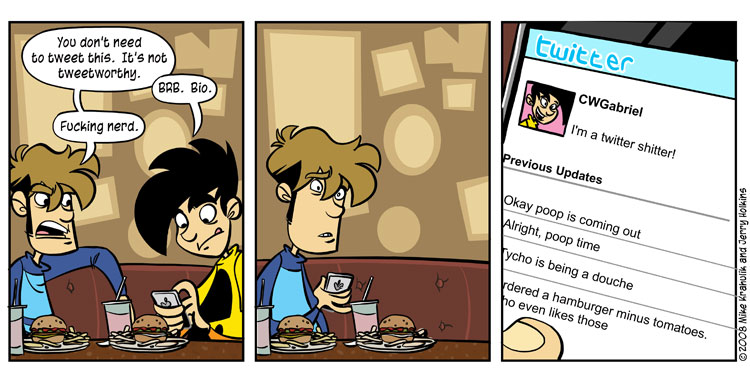
\includegraphics[width=6.00cm, height=3.50cm]{twittershitter}
        \end{center}
}

\begin{frame}[fragile]
    \frametitle{Net::Twitter}
    \begin{itemize}
    \item Uses Moose
    \item Works with Twitter and Identi.ca
    \item REST, Search and Twittervision API support
    \item OAuth and Basic Authentication
    \item 1 to 1 mapping with API
    \item Net::Twitter::Lite
        \begin{itemize}
        \item Fewer Dependencies
        \item Same great taste
        \end{itemize}
    \end{itemize}
\end{frame}

\begin{frame}[fragile]
    \frametitle{Net::Twitter Basic Use}
    \begin{small}
    \begin{verbatim}
    my $nt  = Net::Twitter->new({
                 username => $user,
                 password => $pass,
                 traits   => [qw/API::REST/],
              });
    my $my_tl    = $nt->user_timeline({count=>5});
    my $buddy_tl = $nt->user_timeline({
                        screen_name => $buddy
                    });
    $nt->update('Perl rocks!');
    $nt->new_direct_message($buddy,$tweet);
    $nt->follow_new($cool_tweep);
    $nt->unfollow($seo_guy);

    \end{verbatim}
    \end{small}
\end{frame}


\frame{
    \frametitle{Net::PingFM}
}

\frame{
    \frametitle{WWW::ItsABot}
}

\frame{
    \frametitle{Twitter::TagGrep}
}

\frame{
    \frametitle{Log::Dispatch::Twitter}
}

\frame{
    \frametitle{Twitter $\sim$ Collective Being}
}
\frame{
    \frametitle{}
    Amazing applications wait to be written
    Next Killer App?
}
\end{document}
